\documentclass{article}
\usepackage[utf8]{inputenc}
\usepackage[russian]{babel}
\usepackage{graphicx}
\usepackage{amsmath}
\usepackage{breqn}
\usepackage{wrapfig}
\usepackage{float}
\usepackage{multirow}
\usepackage{caption}
\usepackage{subcaption}

\graphicspath{ {./data/images} }
\author{Александр Романов Б01-107}
\date{}
\title{3.2.4 Свободные колебания в электрическом контуре}

\begin{document}
\maketitle
\section{Введение}
\subsection{Цель работы}
Исследование свободных колебаний в электрическом коле­бательном контуре.
\subsection{В работе используются}
Генератор импульсов, электронное реле, магазин сопротивлений, магазин емкостей, катушка индуктивности, электронный осциллограф, измеритель LRC. 
\begin{figure}[H]
    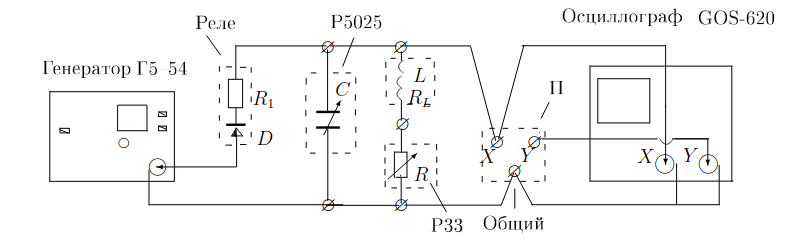
\includegraphics[width=\textwidth]{scheme.png}
    \caption{Схема экспериментальной установки}
    \label{fig:sheme}
\end{figure}

\section{Работа}
\subsection{Измерение периодов свободных колебаний} \label{sec:T}

Соберём cхему, изображённую на Рис. \ref{fig:sheme}.Установим на магазине сопротивлений \(R = 0\); На магазине емкостей
величину \( C = 0.02\; \mu F \). Установим выходное напряжение генератора на \( 28\; V \). По ЭО измерим расстояние между соседними
импульсами \( (x_0 = 2.1 \cdot 5\; ms = 10.5\; ms ) \).

Будем измерять по ЭО расстояние \( x \) , которое занимают \( n \) полных периодов колебаний. Зная период задающих
колебания импульсов \( ( T_0 = 0.01\; s ) \) и \( x_0 \) можно расчитать период колебаний контура \( T \) по формуле:

\[ T = T_0x/(nx_0) \]

Проведём эти измерения изменяя емкость \( C \) от \( 0.02\; \mu F \) до \( 0.9\; \mu F \):

\begin{table}[H]
    \centering
    \label{table:T}
    \begin{tabular}{|c|c|c|c|c|c|c|}
    \hline
    \(C,\; \mu F \) & \(x_0,\; cm\) & \(scale,\; ms\) & \(n\) & \(x,\; cm\) & \(scale,\; ms\)& \(T,\; s\) \\\hline
    0.02   & 2.1    & 5         & 3 & 1     & 1         & 0.0006 \\\hline
    0.13   & 2.1    & 5         & 7 & 3     & 2         & 0.0106 \\\hline
    0.24   & 2.1    & 5         & 5 & 3     & 2         & 0.0274 \\\hline
    0.35   & 2.1    & 5         & 5 & 3.6   & 2         & 0.0480 \\\hline
    0.46   & 2.1    & 5         & 5 & 4.1   & 2         & 0.0718 \\\hline
    0.57   & 2.1    & 5         & 5 & 4.6   & 2         & 0.0999 \\\hline
    0.68   & 2.1    & 5         & 4 & 4     & 2         & 0.1295 \\\hline
    0.79   & 2.1    & 5         & 3 & 3.1   & 2         & 0.1555 \\\hline
    0.9    & 2.1    & 5         & 4 & 4.6   & 2         & 0.1971 \\\hline
    \end{tabular}
\end{table}

\subsection{Критическое сопротивление и декремент затухания}
Приняв \( L = 200\; mH \) рассчитаем ёмкость \( C \), при которой собственная частота колебаний контура 
\( \nu_0 = 1/(2\pi\sqrt{LC}) \) составляет \( 5\; kHz \):

\[ C = 0.005\; \mu F \]

Для полученных значений \( L \) и \( C \) рассчитаем критическое сопротивление контура \( R_{cr} \) по формуле:

\[ R_{cr} = 2\sqrt{L/C} = 12600\; \Omega \]

Установим на магазине ёмкость, близкую к рассчитанной. Будем увеличивать \( R \) от \( 0 \) до \( R_{cr} \). Определим
сопротивление магазина \( R_0 \), при котором контур переходит в апериодический режим:

\[ R_0 = 7400\; \Omega \]

Установим сопротивление \( R \simeq 0.1R_0 \) и будем измерять логарифмический декремент затухающих колебаний
по формуле:

\[ d = \frac{1}{n}\ln \frac{U_k}{U_{k+n}} \]

Повторим эти измерения для разных \( R \) от \( 0.1R_0 \) до \( 0.3R_0 \):

\begin{table}[H]
    \centering
    \begin{tabular}{|c|c|c|c|c|}
    \hline
    \(R,\; \Omega\) & \(n\) & \(U_k,\; cm \)& \(U_{k+n},\; cm\) & \(d\) \\\hline
    740   & 3 & 4    & 1          & 0.462 \\\hline
    986   & 3 & 3    & 0.5        & 0.597 \\\hline
    1232  & 2 & 2.2  & 0.5        & 0.741 \\\hline
    1478  & 2 & 4    & 0.6        & 0.949 \\\hline
    1724  & 2 & 3.4  & 0.4        & 1.070 \\\hline
    1970  & 2 & 3    & 0.3        & 1.151 \\\hline
    \end{tabular}
\end{table}

\subsection{Свободные колебания на фазовой плоскости}
Подключим на ЭО канал Y, на который подано напряжение \( U_R \). Зафиксируем картину:

\begin{figure}[H]
    \centering
    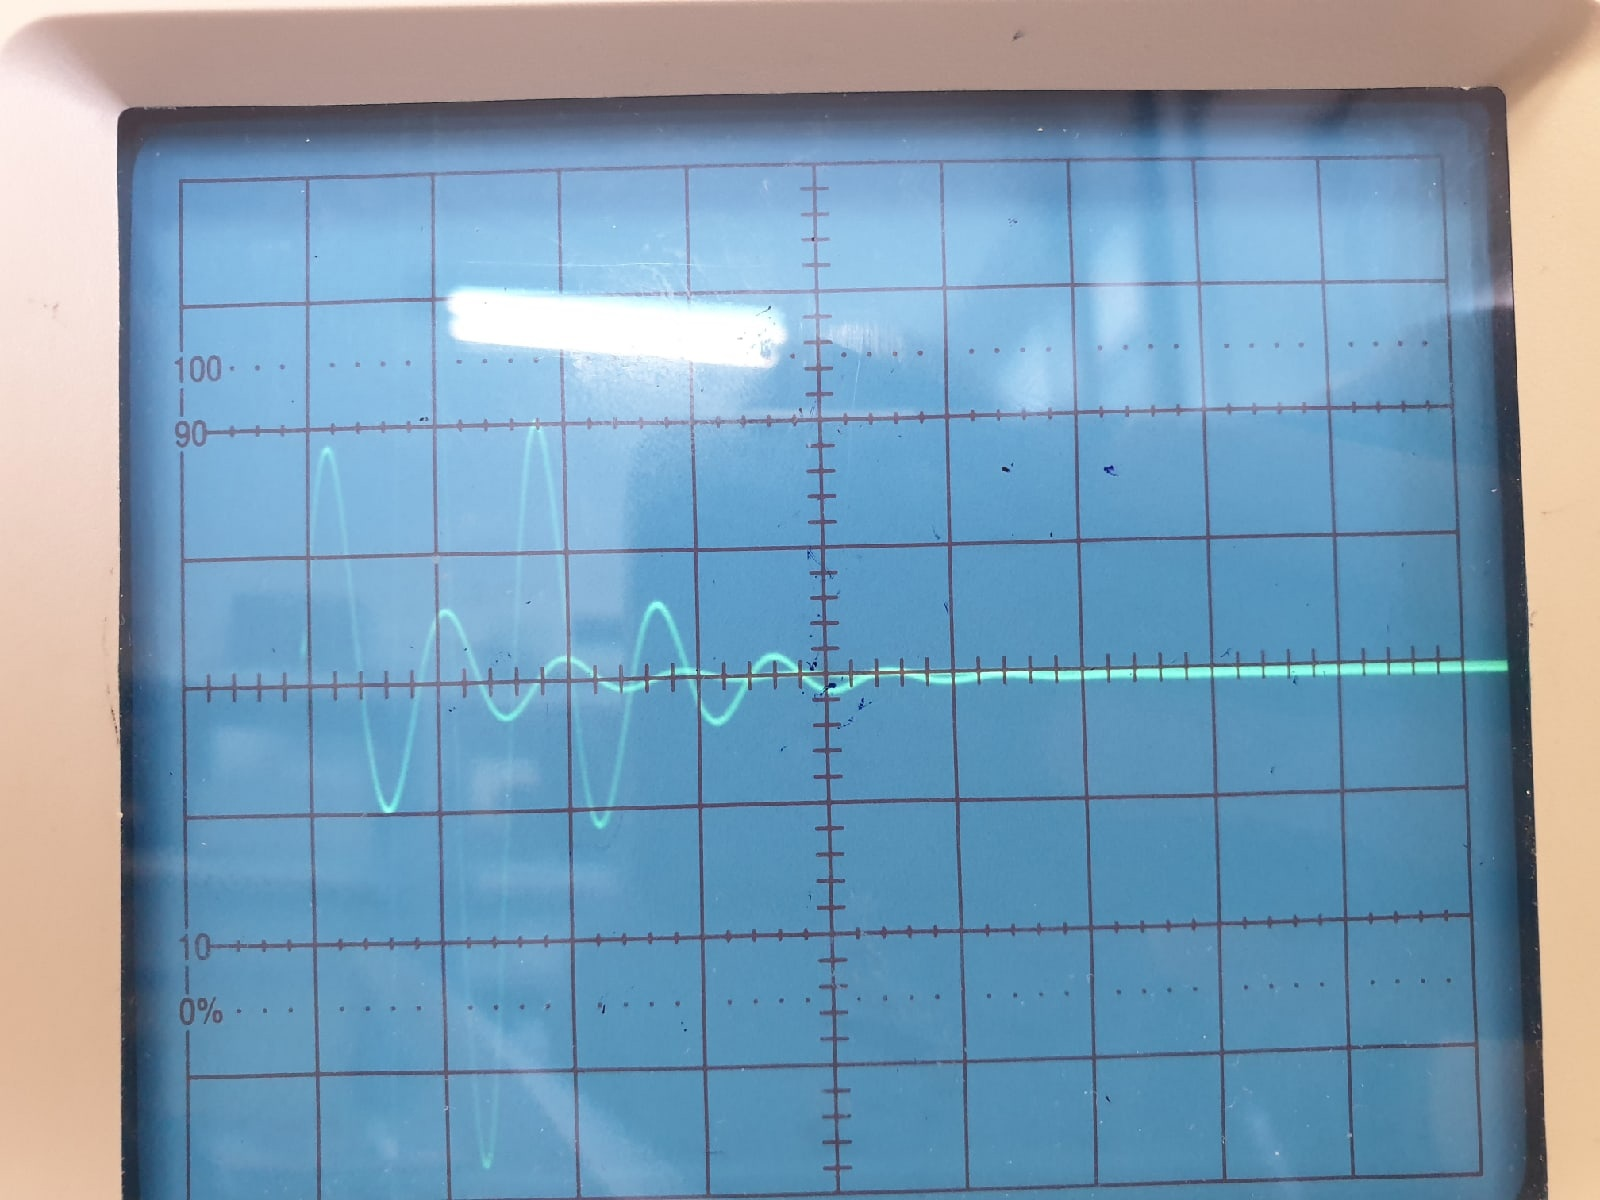
\includegraphics[width = 0.8\textwidth]{X_and_Y_time.jpg}
    \caption{Сигналы X и Y в развёртке по времени}
    \label{fig:XY_time}
\end{figure}

Отключим развёртку по времени, переведы ручку "TIME/DIV" в положение "X-Y".
Будем наблюдать за изменением картины при изменении \( R \) от \(0.1R_0\) до \(0.3R_0\):

\begin{figure}[H]
    \centering
    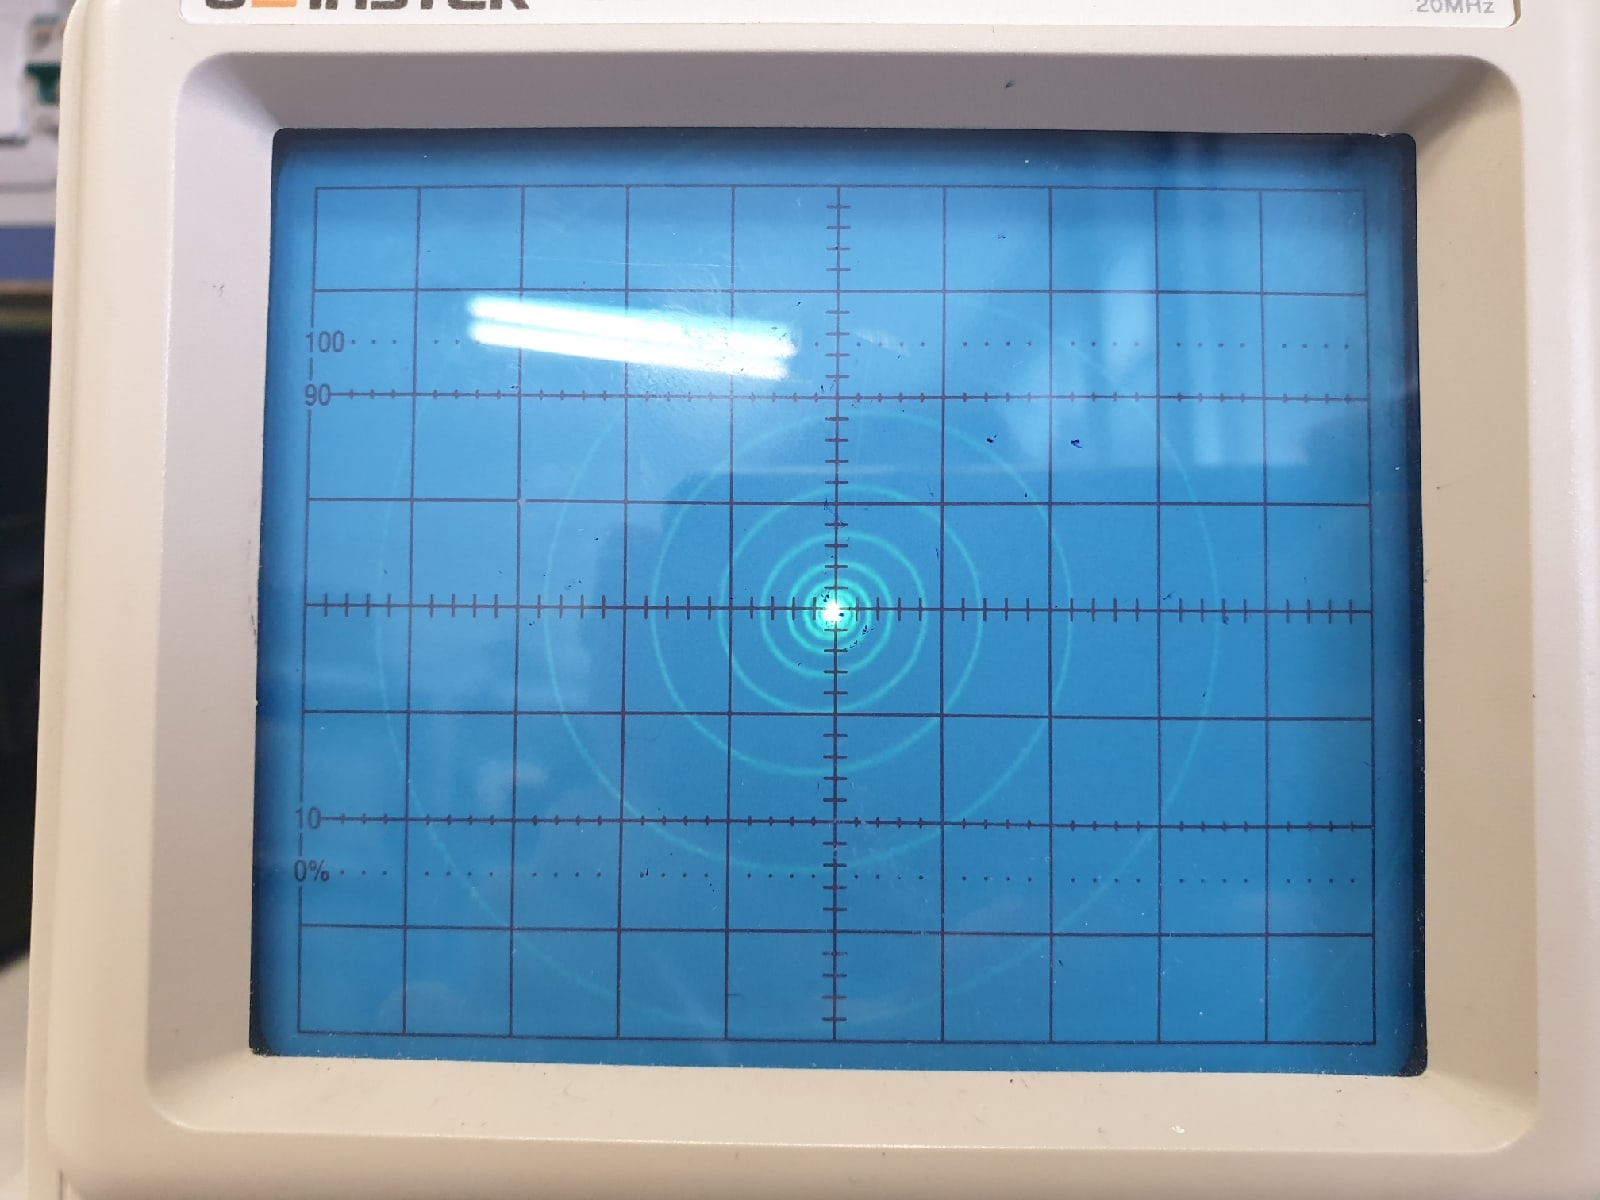
\includegraphics[width = 0.6\textwidth]{XY-740.jpg}
    \caption{Фазовая картина при \(R = 740\; \Omega \)}
    \label{fig:XY_time}
\end{figure}
\begin{figure}[H]
    \centering
    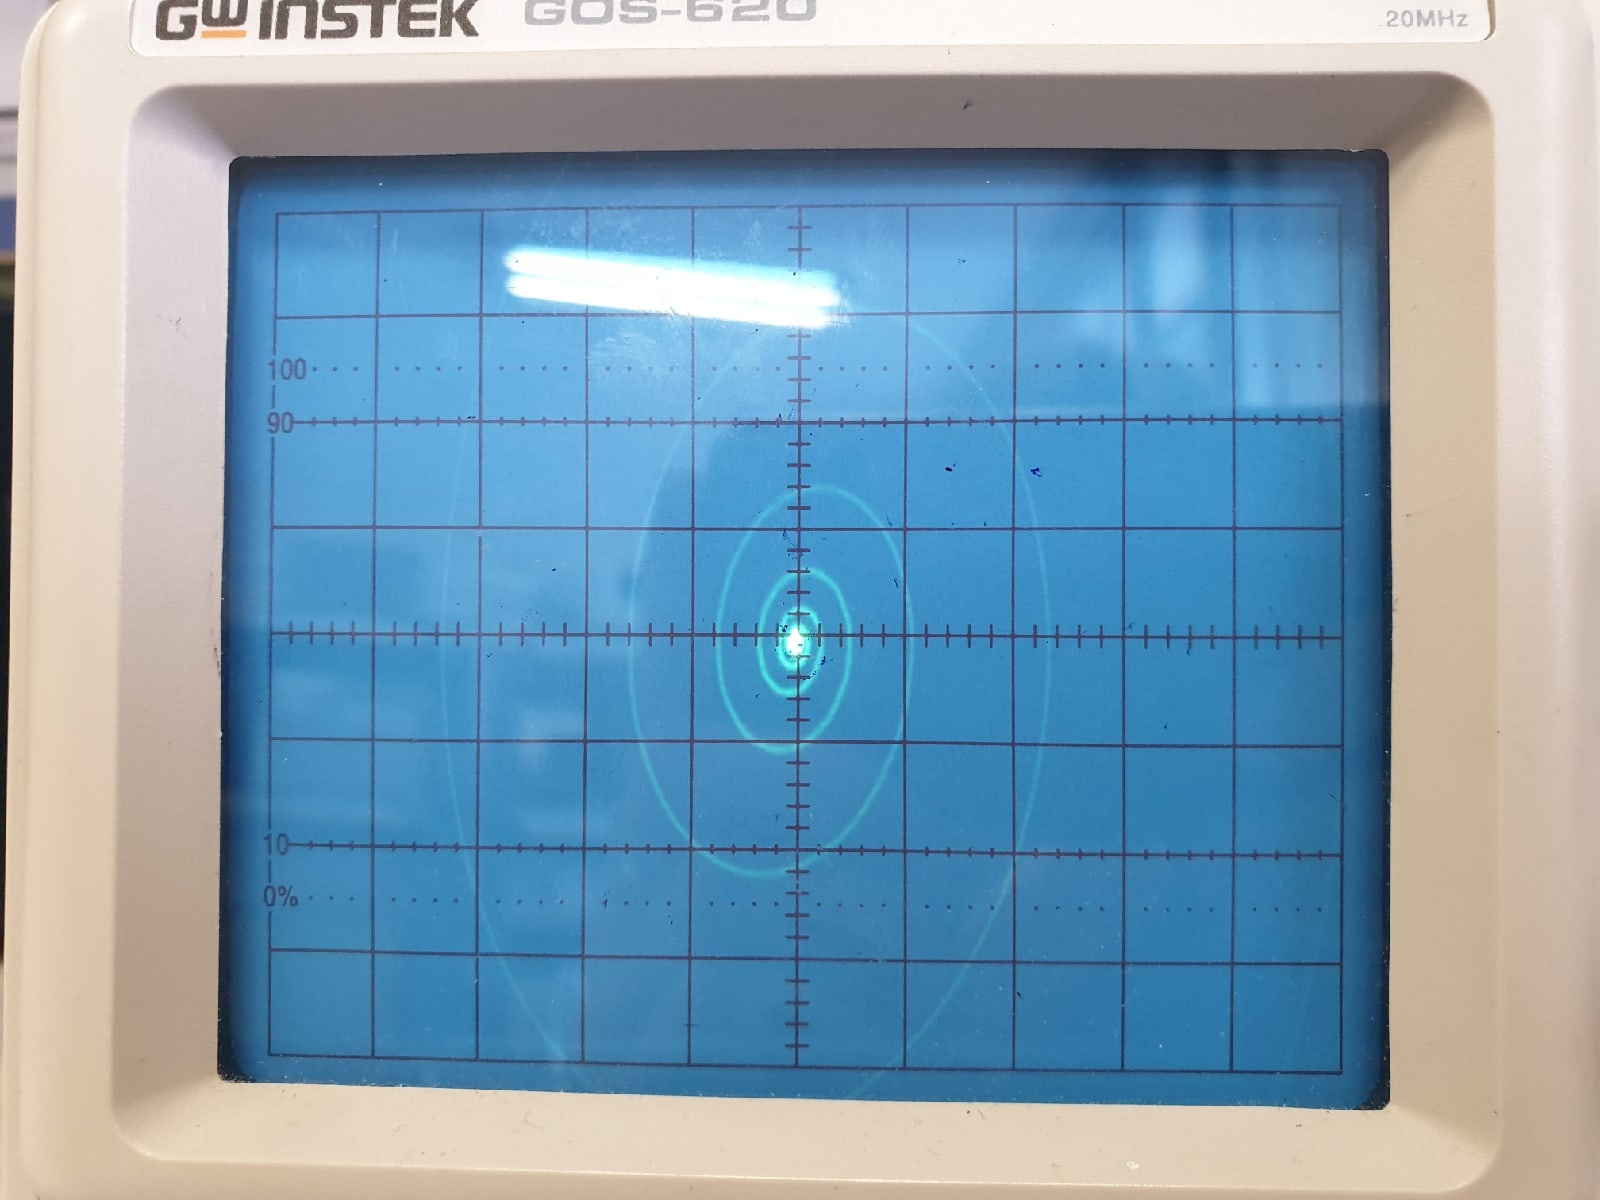
\includegraphics[width = 0.6\textwidth]{XY-1478.jpg}
    \caption{Фазовая картина при \(R = 1478\; \Omega \)}
    \label{fig:XY_time}
\end{figure}
\begin{figure}[H]
    \centering
    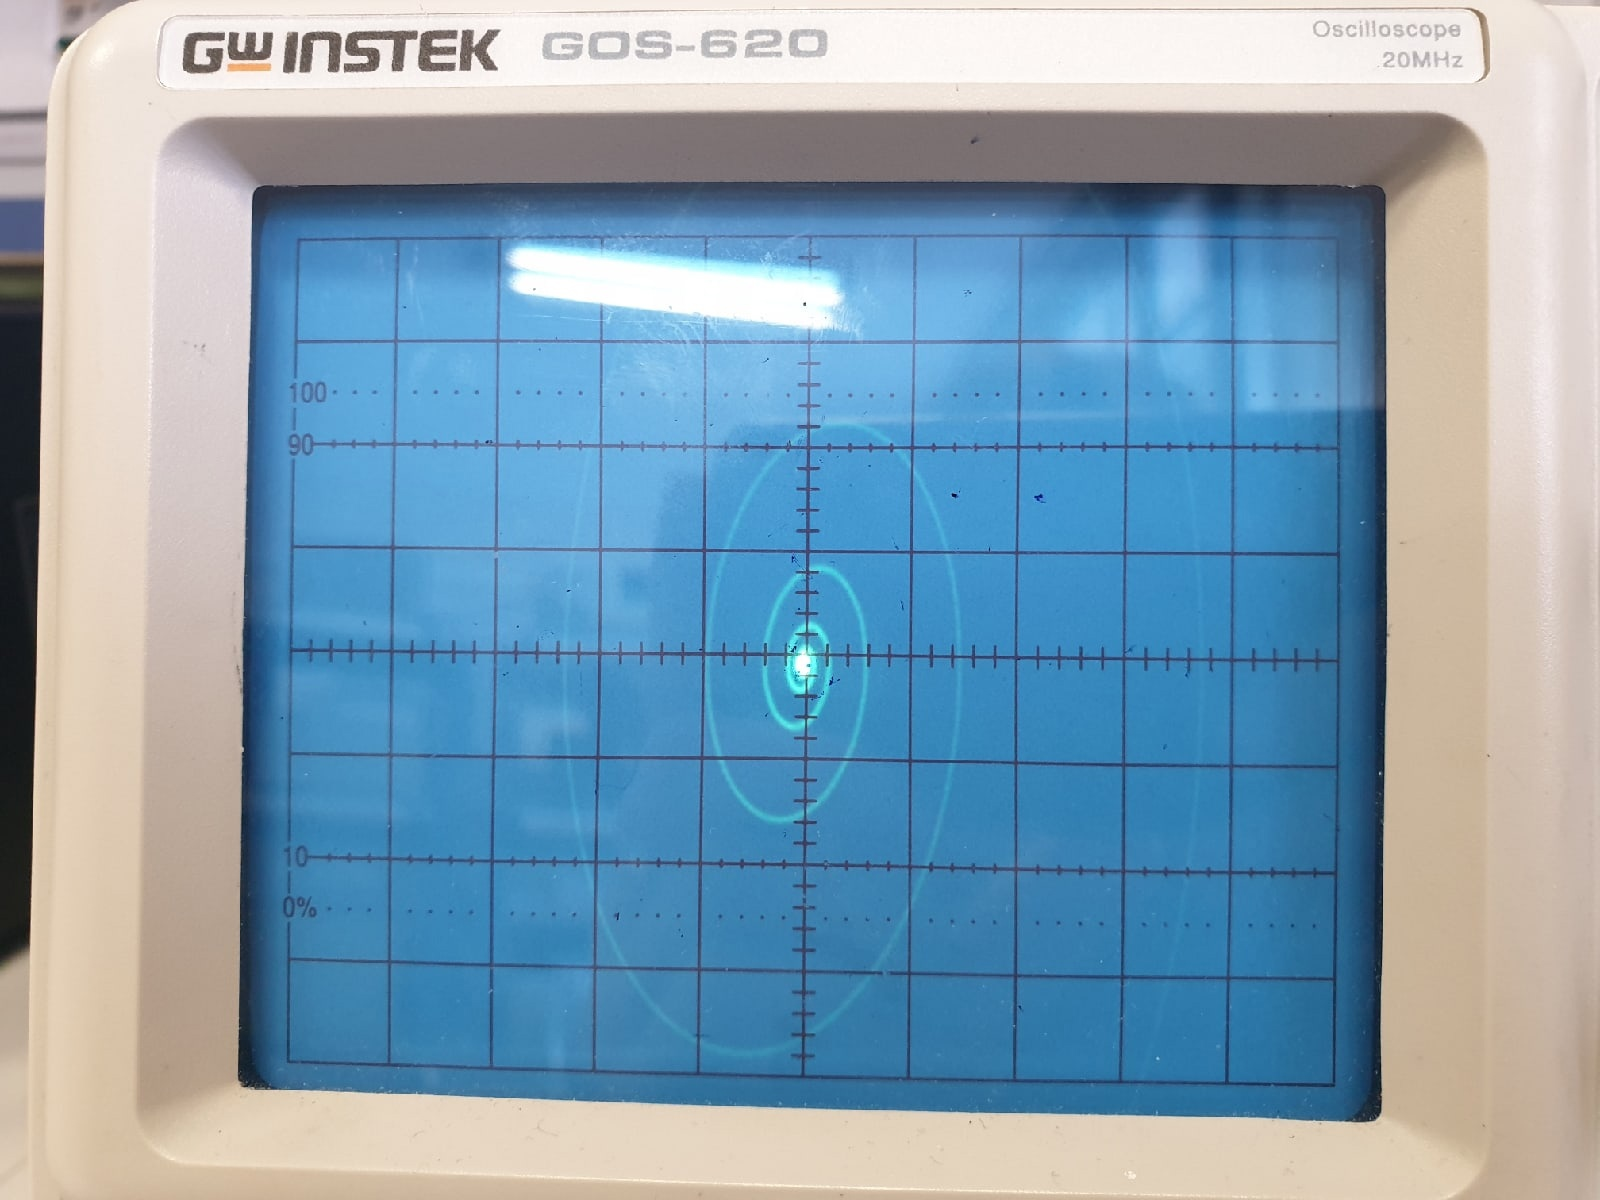
\includegraphics[width = 0.6\textwidth]{XY-1970.jpg}
    \caption{Фазовая картина при \(R = 1970\; \Omega \)}
    \label{fig:XY_time}
\end{figure}

Измерим логарифмический декремент \(d\) контура для максимального и минимального значений \(R\) по формуле:

\[ d = \frac{1}{n}\ln\frac{x_k}{x_{k+n}} \]

\begin{table}[H]
    \centering
    \begin{tabular}{|c|c|c|c|c|}
        \hline
    \(R,\; \Omega\) & \(n\) & \(X_k,\; cm\) & \(X_{k+n},\; cm\) & \(d\) \\\hline
    740  & 2 & 3.5 & 1.4 & 0.458 \\\hline
    1970 & 1 & 2.0 & 0.6 & 1.204 \\\hline
    \end{tabular}
\end{table}

Разберём цепь, отключим катушку и измерим её индуктивность \(L\) и оммическое сопротивление \(R_L\) при помощи
RLC-метра. Получим значения:
\[ L = 146\; mH;\: R_L = 14\;\Omega \]

\section{Обработка экспериментальных данных}
\subsection{Сравнение экспериментальных и теоретических значений периода T}

По формуле \( T = 2\pi\sqrt{LC} \) рассчитаем теоретические значения периодов для контура. и сравним с экспериментальными,
измеренными в пункте \ref{sec:T}:



\section{Выводы}
\end{document}